\documentclass[dvipdfmx,a4paper]{jsarticle}
    \pagestyle{plain}
    \usepackage{amsmath}
    \usepackage{amsthm}
    \usepackage{amssymb}
    \usepackage{graphicx}
    \usepackage{tikz}
    \usepackage{tkz-euclide}
    \usepackage{here}
    \usepackage{cancel}

    \usetikzlibrary{angles}

    \newcommand{\R}{\mathbb{R}}
    \newcommand{\C}{\mathbb{C}}
    \newcommand{\Z}{\mathbb{Z}}
    \newcommand{\N}{\mathbb{N}}
    \newcommand{\Q}{\mathbb{Q}}
    \newcommand{\Lra}{\Leftrightarrow}
    \newcommand{\al}{\alpha}
    \newcommand{\be}{\beta}
    \newcommand{\ga}{\gamma}
    \newcommand{\om}{\omega}
    \newcommand{\De}{\Delta}
    \newcommand{\oraw}{\overrightarrow}
    \newcommand{\bs}{\backslash}
    \newcommand{\2}{I\hspace{-1pt}I}
    \newcommand{\3}{I\hspace{-1pt}I\hspace{-1pt}I}

    \newtheorem{cs}{Case}
    \newtheorem{cas}{Case}
    \newtheorem{case}{Case}
    \newtheorem{apf}{別解}
    \newtheorem{anpf}{別解}

    \usetikzlibrary{calc}
    \title{2022年度京大数学(文系)の解答}
    \author{tt0801}
    \date{\today}
    
    \begin{document}
    \maketitle
    \section{大問1}
    \subsection{問題}
    $5.4 < \log_4 2022 < 5.5$であることを示せ。ただし、$0.301 < \log_{10} 2 < 0.3011$であることは用いてよい。


    \subsection{解答}
    \begin{align*}
        \log_4 2022 &= \dfrac{\log_{10} 2022}{\log_{10} 4} \\
            &= \dfrac{\log_{10} 2 + \log_{10} 1011}{2\log_{10} 2} \\
            &= \dfrac{1}{2} + \dfrac{\log_{10} 1011}{2\log_{10} 2} \ (=A \mathrm{とおく})
    \end{align*}
    である。ここで、$\log_{10} 1011 > \log_{10} 1000 = 3$より、
    \begin{align*}
        A & > \dfrac{1}{2} + \dfrac{3}{2\log_{10} 2} \\
        & > \dfrac{1}{2} + \dfrac{3}{2\cdot 0.3011} \ (\because \log_{10} 2 < 0.3011)\\
        &= \dfrac{33011}{6022} \\
        &> 5.4
    \end{align*}
    なので、$\log_4 2022 > 5.4$である。
    
    また、$\log_{10} 1011 < \log_{10} 1024 = 10 \log_{10} 2$なので、
    \begin{align*}
        A & < \dfrac{1}{2} + \dfrac{10 \log_{10} 2}{2\log_{10} 2} \\
        &= \dfrac{1}{2} + 5\\
        &= 5.5
    \end{align*}
    である。よって、$\log_4 2022 < 5.5$となる。

    以上より、$5.4 < \log_4 2022 < 5.5$が示された。


    \subsection{解説}
    $\log_{10} 2$の評価式が与えられているので、$\log_{10} 2$を作ることを意識して式変形をする。

    \section{大問2}
    \subsection{問題}
    下図の三角柱$\mathrm{ABC - DEF}$において、Aを始点として、辺に沿って頂点を$n$回移動する。すなわち、
    この移動経路
    \begin{equation*}
        \mathrm{
            P_0 \rightarrow P_1 \rightarrow P_2 \rightarrow \cdots 
            \rightarrow P_{n-1} \rightarrow P_n \quad (\mathrm{ただし} P_0 = A)
        }
    \end{equation*}
    において、$\mathrm{P_0P_1, P_1P_2, \cdots, P_{n-1}P_n}$はすべて辺であるとする。また、
    同じ頂点を何度通ってもよいものとする。このような移動経路で、終点$\mathrm{P_n}$が
    $\mathrm{A, B, C}$のいずれかとなるものの総数$a_n$を求めよ。

    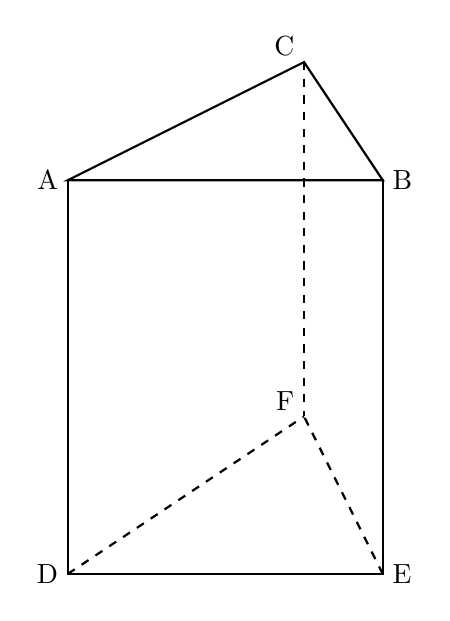
\begin{tikzpicture}
        % Draw the base square A - B - E - D
        \draw[thick] (0,0) -- (4,0) -- (4,-5) -- (0,-5) -- cycle;

        % Draw the top triangle A - C - B
        \draw[thick] (0,0) -- (3,1.5) -- (4,0) -- cycle;

        % Connect base to apex of the triangle C - F
        \draw[thick, dashed] (3,1.5) -- (3,-3);

        % Draw the diagonal lines of the base D - F, E - F
        \draw[thick, dashed] (0,-5) -- (3,-3);
        \draw[thick, dashed] (4,-5) -- (3,-3);

        % Label the points
        \node[anchor=east] at (0,0) {A};
        \node[anchor=west] at (4,0) {B};
        \node[anchor=east] at (3,1.7) {C};
        \node[anchor=east] at (0,-5) {D};
        \node[anchor=west] at (4,-5) {E};
        \node[anchor=east] at (3,-2.8) {F};
    \end{tikzpicture}

    \subsection{解答}

    \subsection{解説}


\end{document}